Malgré l'ajout d'un partage de poids dans le réseau $\mathcal{S}$MorphNetTanh, certaines expériences restent un échec dans le cadre d'une opération cible d'ouverture ou de fermeture : le réseau aura convergé vers un minimum local. Dans ces échecs, c'est à la fois l'aspect visuel du noyau des couches qui est considéré comme trop éloigné de la forme de la fonction structurante cible, et à la fois les métriques d'évaluation des performances du réseau qui sont considérées comme mauvaises par rapport aux succès. Les poids des noyaux $w$ des couches du réseau, avec les paramètres de contrôle $\alpha$ associés, étant responsables des bonnes ou mauvaises performances du réseau. \\
%Les poids des noyaux $w$ et les paramètres de contrôle $\alpha$ des couches étant responsables des bonnes ou mauvaises performances du réseau.

\vspace{-1.6mm}
En analysant, sur ces échecs, les poids des couches du réseau, que ce soit le noyau $w$ ou le paramètre $\alpha$, on observe le manque d'une certaine harmonie : d'un côté, les poids dans les noyaux $w$ sont très étalés sur le support, et leurs valeurs tournent autour de la moyenne et manquent d'une certaine binarisation, surtout aux bords du support, rendant difficile la distinction d'un << objet >> par rapport au << fond >> du suppport ; et d'un autre côté, on remarque que la valeur des pramètres de contrôle $\alpha$ sont très proches de $0$, ne générant que des pseudo-opérations morphologiques, et sont bien souvent du mauvais signe (ils ne prennent pas la << bonne >> opération cible). Une idée est alors de créer une << influence >> sur ces poids, qui puisse les guider vers la structure souhaitée, sans donner des informations trop précises sur la structure cible. \\

\vspace{-1.6mm}
Cette << influence >>-là se base sur le même concept que celui utilisé pour le partage de poids doux : on ajoute, dans la fonction de perte \textit{loss}, une métrique de contrainte sur les poids de couches visés, pondérée par un hyperparamètre $\lambda$ (voir formule \ref{MSEpConstraintFilters}). Cette contrainte, fonction définie sur les poids $w / \alpha$ à valeurs dans $\mathbb{R}$, doit illustrer l'erreur sur l'<< aspect >> que l'on souhaite ajouter dans les poids du réseau. Il peut s'agir d'un aspect géométrique, d'un aspect morphologique, ou encore d'une distance. En ajoutant cette contrainte dans la \textit{loss}, le réseau va alors se forcer à minimiser cette contrainte lors de son entraînement, faisant tendre les poids vers l'aspect souhaité.  \\


\noindent \textbf{Attention : } 
Ces contraintes-là sont appliquées uniquement dans des cas particuliers où l'on fait une hypothèse forte sur l'aspect des noyaux $w$ et des paramètres $\alpha$ des couches du réseau. Elles sont utilisées seulement dans des contextes où on a des hypothèses sur la forme des poids des couches qui peuvent être justifiées, où l'on sait que la contrainte doit être respectée et est pertinente dans le cas en question. Si on ne sait rien à priori sur la forme des poids que l'on cherche, elles ne sont pas pertinentes. \\


On distingue ici deux types de contraintes sur les réseaux morphologiques : les contraintes géométriques sur les noyaux $w$, et les contraintes sur les paramètres de contrôle $\alpha$. Ces deux types de contraintes sont étudiés dans les pages suivantes.





\newpage




%\setbox1=\hbox{$\bullet$}\setbox2=\hbox{\tiny$\bullet$}
%\setlength{\mylen}{\dimexpr0.5\ht1-0.5\ht2}

\vspace{-1.6mm}
Mais avant de plonger dans ces métriques et de voir leur impact sur la forme des noyaux et plus généralement sur la convergence des réseaux, rappelons qu'il est important que les fonctions associées soient continues partout, et, si possible, dérivables partout, afin de pouvoir calculer le gradient de la \textit{loss} par rapport aux poids du réseau, nécessaire à la rétropropagation du gradient lors de l'entraînement. \\

\vspace{-2.0mm}
\noindent L'application $| \hspace{1.0mm} \text{\raisebox{\mylen}{\tiny$\bullet$}} \hspace{1.0mm} |^\zeta : \mathbb{R} \rightarrow \mathbb{R}$, définie pour $\zeta \in \mathbb{R}$, et qui à un réel $x$ associe $|x|^\zeta$, est beaucoup utilisée dans les différentes métriques de contraintes citées. Étudions donc d'abord rapidement ses propriétés de continuité et de dérivabilité sur $\mathbb{R}$ en fonction de $\zeta \in \mathbb{R}$. On cherche en particulier à connaître les conditions nécessaires et suffisantes sur le paramètre $\zeta$ pour que l'application $x \mapsto |x|^\zeta$ soit dérivable partout sur $\mathbb{R}$. \\

\vspace{-0.2mm}
\noindent \underline{Sur $\mathbb{R}^*$ :} \\

\vspace{-0.8mm}
\noindent On sait que l'application $x \mapsto x^\zeta$ est continue et dérivable sur $\mathbb{R}_+^*$ pour tout $\zeta \in \mathbb{R}$. Sur $\mathbb{R}_+^*$, l'application $x \mapsto |x|^\zeta$ devient $x \mapsto x^\zeta$, qui est donc continue et dérivable $\forall \zeta \in \mathbb{R}$. Sur $\mathbb{R}_-^*$, $x \mapsto |x|^\zeta$ devient $x \mapsto (-x)^\zeta$, qui est également continue et dérivable $\forall \zeta \in \mathbb{R}$, puisque $\forall x \in \mathbb{R}_-^*, -x \in \mathbb{R}_+^*$. Ainsi, $x \mapsto |x|^\zeta$ est continue et dérivable sur $\mathbb{R}^*$, $\forall \zeta \in \mathbb{R}$. \\

\vspace{-0.2mm}
\noindent \underline{En $0$ :} \\

%\vspace{-2.0mm}
%\noindent Continuité en $0$ : \\

\vspace{-0.8mm}
\noindent On sait que, sur $\mathbb{R}_+$, l'application $x \mapsto x^\zeta$ n'est pas définie en $0$ pour $\zeta \in \mathbb{R}_-^*$, car $x^\zeta$ tend vers $+\infty$ quand $x$ tend vers $0^+$ si $\zeta<0$. Si $\zeta=0$, l'application $x \mapsto x^\zeta$ définie sur $\mathbb{R}_+^*$ peut être prolongée par continuité en $0$, avec $x^\zeta = 1$ en $x=0$, car $\forall x \in \mathbb{R}_+^*, x^0=1$. Enfin, si $\zeta \in \mathbb{R}_+^*$, l'application $x \mapsto x^\zeta$ est bien définie et continue sur $\mathbb{R}_+$, et donc en $0$. Ainsi, l'application $x \mapsto |x|^\zeta$ est définie et continue en $0$ si et seulement si $\zeta \geq 0$. \\

\vspace{-1.0mm}
\noindent Étudions à présent la dérivabilité de $x \mapsto |x|^\zeta$ en $0$, en partant de la définition-même de la dérivabilité.
Soit $\zeta>0$ (excluons le cas $\zeta=0$ pour l'instant), et soit $h>0$.

\vspace{1.0mm}
\noindent À gauche : $\frac{|0-h|^\zeta - |0|^\zeta}{0-h-0} = \frac{|-h|^\zeta - |0|^\zeta}{-h} = \frac{|-h|^\zeta}{-h} = \frac{h^\zeta}{-h} = -h^{\zeta-1} $

\vspace{1.0mm}
\noindent À droite : $\frac{|0+h|^\zeta - |0|^\zeta}{0+h-0} = \frac{|h|^\zeta - |0|^\zeta}{h} = \frac{|h|^\zeta}{h} = \frac{h^\zeta}{h} = h^{\zeta-1}$

\vspace{1.0mm}
\noindent L'application $x \mapsto |x|^\zeta$ est donc dérivable en $0$ \underline{ssi} : $\lim_{h \rightarrow 0^+} \left ( -h^{\zeta-1} \right ) = \lim_{h \rightarrow 0^+} \left ( h^{\zeta-1} \right )$.

\noindent Donc, si $\zeta \neq 0$, elle est dérivable en $0$ \underline{ssi} $\zeta>1$. Si $\zeta=0$, elle est également dérivable en $0$ (en considérant le prolongement par continuité en $0$).

\vspace{5.0mm}
\noindent $\Rightarrow$ L'application $x \mapsto |x|^\zeta$ est donc dérivable partout sur $\mathbb{R}$ \underline{ssi} $\zeta > 1$ ou $\zeta=0$. \\


\vspace{1.6mm}
La figure \ref{fig:powered_absolute_curves} ci-après illustre la courbe de la fonction $x \mapsto |x|^\zeta$ pour quelques valeurs de $\zeta$. Elle permet de comprendre facilement le comportement et l'évolution de cette application en fonction de la valeur de $\zeta$. On constate l'applatissement de la courbe en $0$ quand $\zeta$ augmente, et on devine bien la dérivabilité en $0$ pour $\zeta > 1$.



\newpage

% Illustrations
%\vspace{0.6mm}
\begin{figure}[htp]
  \begin{center}
    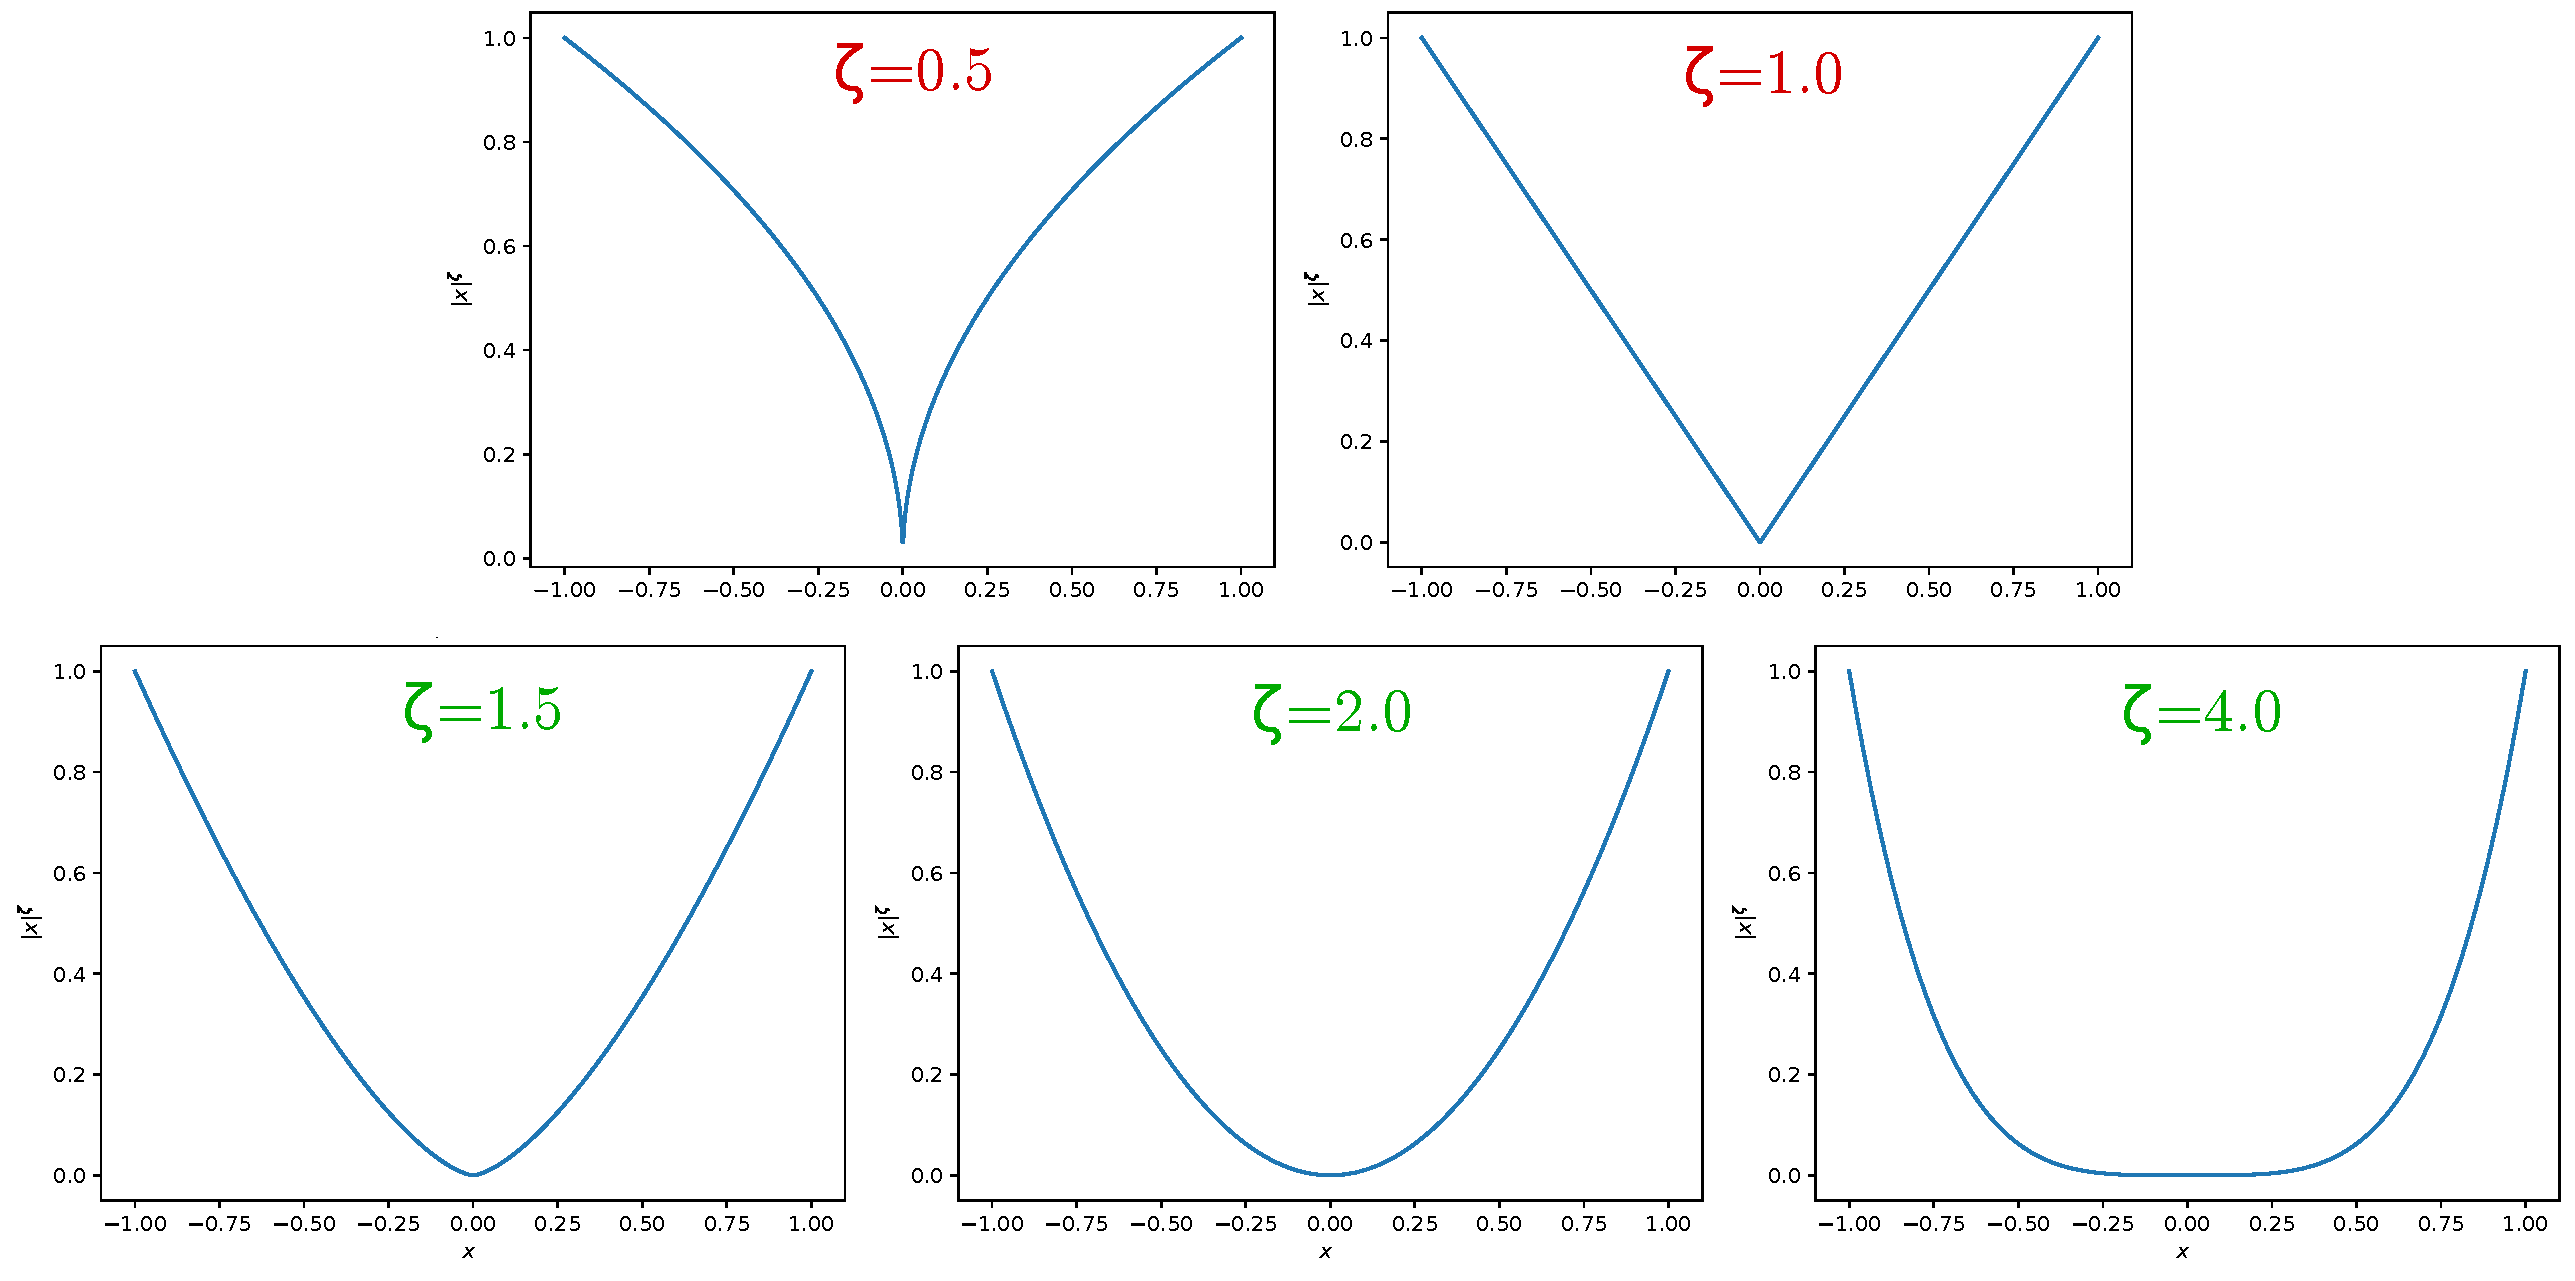
\includegraphics[width=0.80\linewidth]{parts/3-contributions/C-contraintes_geometriques/figures/curves.pdf}
    %\vspace{-1.0mm}
    \caption{ \centering Courbes de la fonction $x \mapsto |x|^\zeta$ dans l'intervalle $[-1,1]$, pour différentes valeurs de $\zeta$. En-haut : non dérivable en $0$ ($1 \geqslant \zeta > 0$) ; en-bas : dérivable en $0$ ($\zeta > 1$).}
    \label{fig:powered_absolute_curves}
  \end{center}
\end{figure}


% Explications

\vspace{-4.0mm}
\noindent La propriété de cette application $x \mapsto |x|^\zeta$ d'être dérivable partout, en particulier en $x=0$, si et seulement si $\zeta>1$ (ou $\zeta=0$, mais ce cas ne sera jamais utilisé) justifient, dans les métriques suivantes, l'utilisation par défaut de $\zeta=2$ dans les fonctions mises en puissance. Cette propriété est également valable pour la norme euclidienne dans un espace à $n$ dimensions, d'où le fait que $\zeta$ soit aussi égal à $2$ par défaut dans les formules \ref{erreur_center} et \ref{erreur_disp} de la première et de la deuxième contrainte géométrique (ci-après).


